\chapter{System-Design}
\label{cha:systemdesign}

\section{Architektur des dezentralen Identitätsmanagementsystems}

\subsection{Entscheidung über Framework}
Um sich für eine Architektur festzulegen, muss zunächst die Entscheidung über die darunterliegende Plattform getroffen werden. Dabei stehen die in Kapitel 5 betrachteten Lösungen zur Auswahl: Luniverse, Dock, PolygonId, Sovrin und Shocard. Für die Entwicklung des Prototypen wird im folgenden :
\begin{itemize}
	
	\item Polygon (als unterliegende Blockchain) zeigt folgende Vorteile auf \cite{ID54}:
	\begin{itemize}
		\item Die Blockchain skaliert hervorragend mit einer steigenden Anzahl von Transaktionen
		\item Geringe Transaktionskosten
		\item Hohe Interoperabilität mit Ethereum
		\item Etablierte Plattform und weite Verbreitung im Markt
	\end{itemize}
	
	\item PolygonId:
	\begin{itemize}
		\item Möglichkeit zum Widerruf von Informationen gegeben
		\item Informationen sind überprüfbar
		\item Selektive-Disclosure implementierbar
		\item Alle nicht-funktionalen Anforderungen implementierbar
		\item Unterstützt W3C Standard für VC's
		\item Credential Exchange erfolgt nach Identity-Foundation Standard
	\end{itemize}
\end{itemize}
\subsection{Grobe Architektur}
Prinzipiell besteht die Architektur aus drei Komponenten: Einem Verifier, einem Issuer und dem Holder. Jede dieser drei Komponenten laufen unabhängig voneinander und können mit fremd-implementierten Instanzen kommunizieren. Das hier dargestellte Szenario ist das Erstellen, Übertragen und Verifizieren von einem digitalen Führerschein auf der Blockchain. Die System-Architektur sieht dabei wie folgt aus:
\begin{figure}[h]
	\centering
	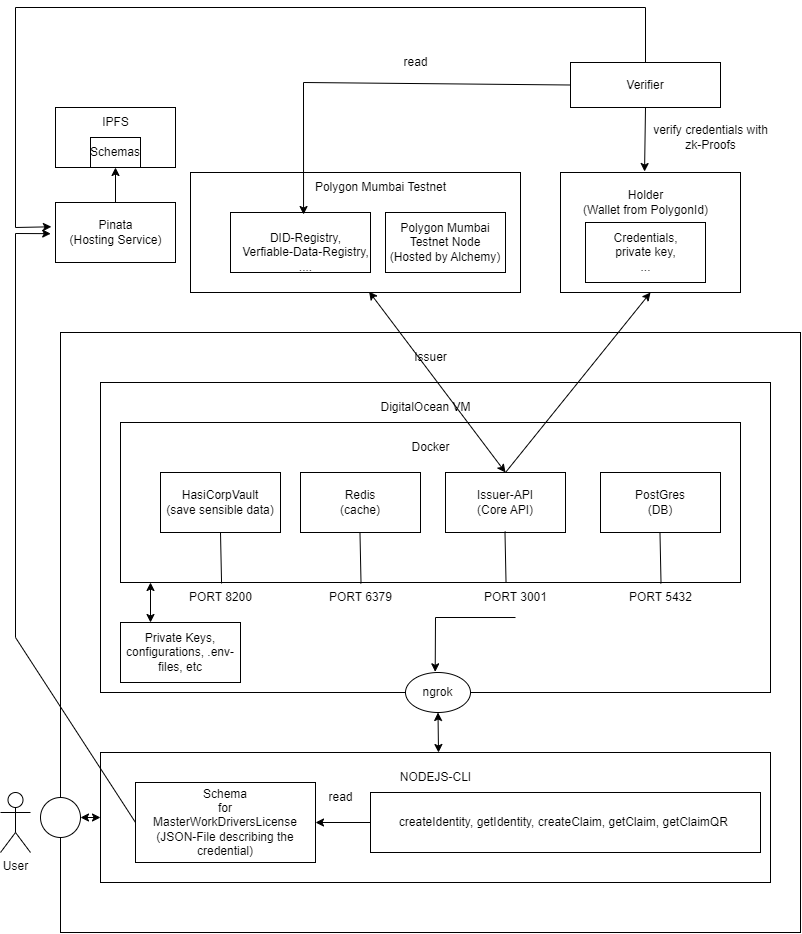
\includegraphics[scale=0.4]{media/system-design}
	\caption{System-Design des Prototyps}
	\label{fig:meine-grafik}
\end{figure}
Es ist zu erkennen, dass der Issuer die zentrale Komponente ist. Um den Issuer zu hosten wird eine virtuelle Maschine von DigitalOcean \footnote{https://www.digitalocean.com/} verwendet. VMs werden bei DigitalOcean auch Droplets genannt, wobei das Droplet für den Prototypen wie folgt konfiguriert ist:
\begin{figure}[h]
	\centering
	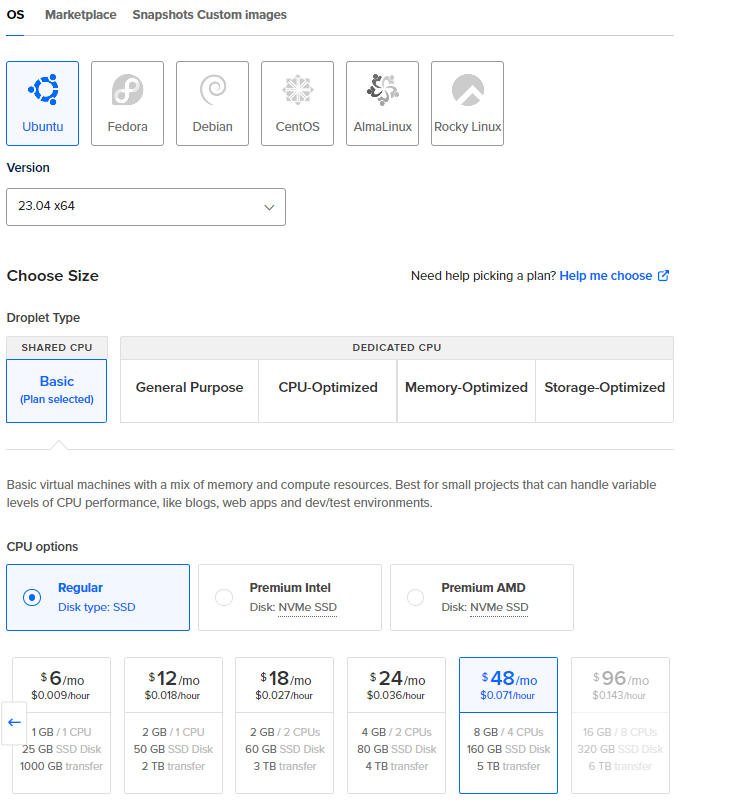
\includegraphics[scale=0.4]{media/config}
	\caption{Konfiguration des DigitalOcean-Droplets}
	\label{fig:meine-grafik}
\end{figure}
Auf dem Droplet läuft ein Docker der alle in der Grafik darstellen Container orchestriert. Der einzige Container, der auch von extern erreichbar sein muss ist der 'issuer-api'-Container, da er die REST-API Anfragen erhält. Für Letzteres wird 'ngrok' \footnote{https://ngrok.com/} verwendet, wobei ein Tunnel von einer öffentlichen IP auf den Lokalhost des Droplets gebaut wird. Dieser Tunnel wird vom NodeJs-Cli verwendet, um Anfragen über die API an den - von Alchemy \footnote{https://www.alchemy.com/} gehosteten - Netzwerk-Knoten weiterzuleiten. Die Schemas müssen öffentlich zugänglich sein, da sie unter anderem im Verifier und Issuer referenziert werden. Um dem ursprünglichen Gedanken der Dezentralität treu zu bleiben werden auch die Schemas dezentral - über IPFS \footnote{https://ipfs.tech/} - gespeichert. Als Schnittstelle zwischen IPFS und der Anwendung wird Pinata \footnote{https://www.pinata.cloud/} verwendet. Das dort gehostete Schema sieht hierbei wie folgt aus:
\begin{lstlisting}[language=json,firstnumber=1]	
		[...]
		"MasterWorkDriversLicense": {
			"@context": {
			 [...]
				"TypeOfVehicle": {
					"@id": "polygon-vocab:TypeOfVehicle",
					"@type": "xsd:string"
					[...]
					
					"enum": [
						"Car",
						"Truck",
						"Scooter",
						"Motorcycle"
					],
					
				},
				"YearOfReceipt": {
					"@id": "polygon-vocab:YearOfReceipt",
					"@type": "xsd:integer"
				}
			},
			[...]
		}
	}
	]
}
\end{lstlisting}
Es ist zu erkennen, dass der Führerschein für den Prototypen aus zwei Attributen besteht:
\begin{itemize}
	\item YearOfReceipt: Ein Integer, der das Jahr darstellt an dem der Holder den Führerschein erworben hat
	\item TypeOfVehicle: Ein String, der den Typ des Vehicle beschreibt. Hierbei gibt es vier Typen: 
	
	\begin{itemize}
		\item Car
		\item Truck
		\item Scooter
		\item Motorcycle
	\end{itemize}
\end{itemize}

Zum Erstellen der Schemata stellt PolygonId einen Schema-Builder zur Verfügung \footnote{https://schema-builder.polygonid.me/}. \\
Nachdem der Issuer den Führerschein ausgestellt hat kann der Holder ihn entgegennehmen. Der nächste Schritt ist, dass ein Verifier einen Query definiert, der wie folgt aussehen könnte:
\begin{lstlisting}[language=json,firstnumber=1]
{[...]
	id: 1,
	circuitId: 'credentialAtomicQuerySigV2', // algorithmus zum Erstellen des zk-Proofs
	query: {
		allowedIssuers: ['*'],
		type: 'MasterWorkDriversLicense', // im Schema definierter Typ
		context: 'https://ipfs.io/ipfs/QmTSd6saivXHysRopQdM1yswp2qyFwobL7fwuFpkVTS8gd',
		credentialSubject: {
			YearOfReceipt: {
				$lt: 2022,
			},
		},
	},
	[...]
}
\end{lstlisting}
Der hier dargestellte Query überprüft primär, ob der Führerschein des Holders älter als vom Jahr 2022 ist. Indirekt fragt er ebenso ab, ob der Nutzer den beschriebenen Credential besitzt und ob dieser noch gültig ist. Ist dies der Fall, so wird der zk-Proof an den Verifier gesendet.

\section{Der Issuer}
Der Issuer kann im Polygon-Framework auf zwei Weisen realisiert werden:
\begin{itemize}
	\item 'On-Chain': Das Ausgabe der Credentials geschieht hierbei 'on-chain', also innerhalb der Blockchain. Implementiert wird die Logik mittels Smart-Contracts, was bedeutet, dass die Logik beliebig erweitert werden kann. Die anzuwendende Programmiersprache ist Solidity \footnote{https://soliditylang.org/}, was der gleichen Sprache entspricht wie im Ethereum Ökosystem. Durch die Smartcontracts werden - die in \nameref{technischeDatenPolygon} erwähnten - Zustandsbäume gespeichert. Auch Identitäten können so generiert  werden. In der Dokumentation werden zwei Szenarien besprochen: öffentliche und private Anwendungsfälle, die beide in der Blockchain realisiert werden können. Auch wenn der Issue-Prozess in der Blockchain stattfindet, so werden private Credentials nicht on-chain generiert. Dies passiert offline und ein Beweis für die Validität wird in der Blockchain gespeichert.
	\item  'Off-Chain': Hierbei werden die Credentials in einem Issuer-Knoten erstellt, der eine API zur Verfügung stellt. Um den Knoten zu hosten wird ein Droplet von 'Digital Ocean' verwendet,  welches sich in Frankfurt befindet. Nachdem die Knoten-Software installiert wurde und alle Parameter konfiguriert wurden (privater Schlüssel von Issuer, CPU-Typ, URL's, Export von Variablen, RPC-Endpunkt-URL, usw). Für letzteren Endpunkt können öffentliche Knoten verwendet werden wie etwa 'https://rpc-mumbai.matic.today'. Dieser ist jedoch vergleichweise langsam und es gehen Vorteile von privaten Endpunkten verloren wie Monitoring und bessere Debugging-Möglichkeiten. Aus diesen Gründen wird Alchemy (https://www.alchemy.com/) verwendet. Der private Schlüssel wird aus Sicherheitsgründen in einem Tool zur Speicherung sensibler Daten verwendet (Vault by HashiCorp \label{vault}). Redis (https://redis.io/) wird als Cache verwendet. Letzten drei Komponenten sind jeweils in einem Container in Docker (https://www.docker.com/). In einem vierten Container befindet sich ein Server, der über eine REST-API Endpunkte zur Verfügung stellt. Die für diesen Prototypen relevanten Aktivitäten sind das Generieren und Lesen von Identitäten, Das Erstellen und Schreiben von Claims und das generieren von QR-Codes, die der potentielle Holder mit seiner Wallet-App scannen kann. Alle die zuletzt genannten Funktionen wurden in einem CLI (Command Line Interface) in Python zur Verfügung gestellt. Dabei werden in Abbildung \ref{fig:CLI} die Befehle mit einem jeweiligen Beispiel illustriert.
	
	\begin{figure}[t]
		\centering
		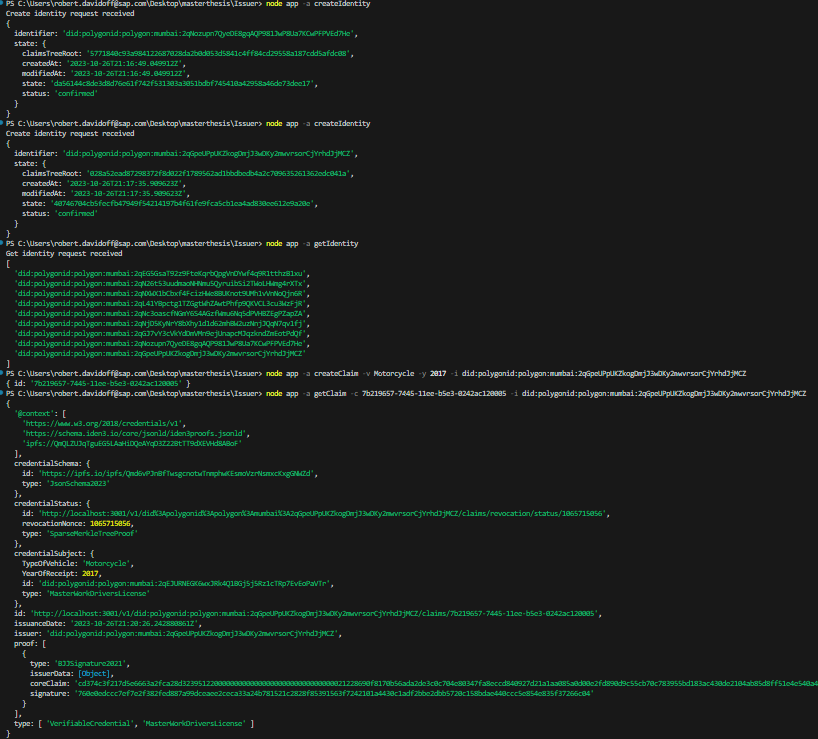
\includegraphics[scale=0.7]{media/CLI}
		\caption{CLI Beispiele}
		\label{fig:CLI}
	\end{figure}
	
	Alle Implementierungen verwenden intern die REST-API des Issuer-Knoten, der über ngrok öffentlich zugänglich ist. Alternativ ist es möglich dem Droplet eine 'reserved IP' zuzuweisen. Mittels PolygonScan (https://mumbai.polygonscan.com) und dem Monitoring Tool bei Alchemy sind die Aktivitäten auch als Transaktionen einsehbar. Nachdem der QR-Code gescannt wurde, kann man in der App den Credential einsehen, was in Abbildung \ref{fig:appCredential} ersichtlich wird.
	 \begin{figure}[t]
	 	\centering
	 	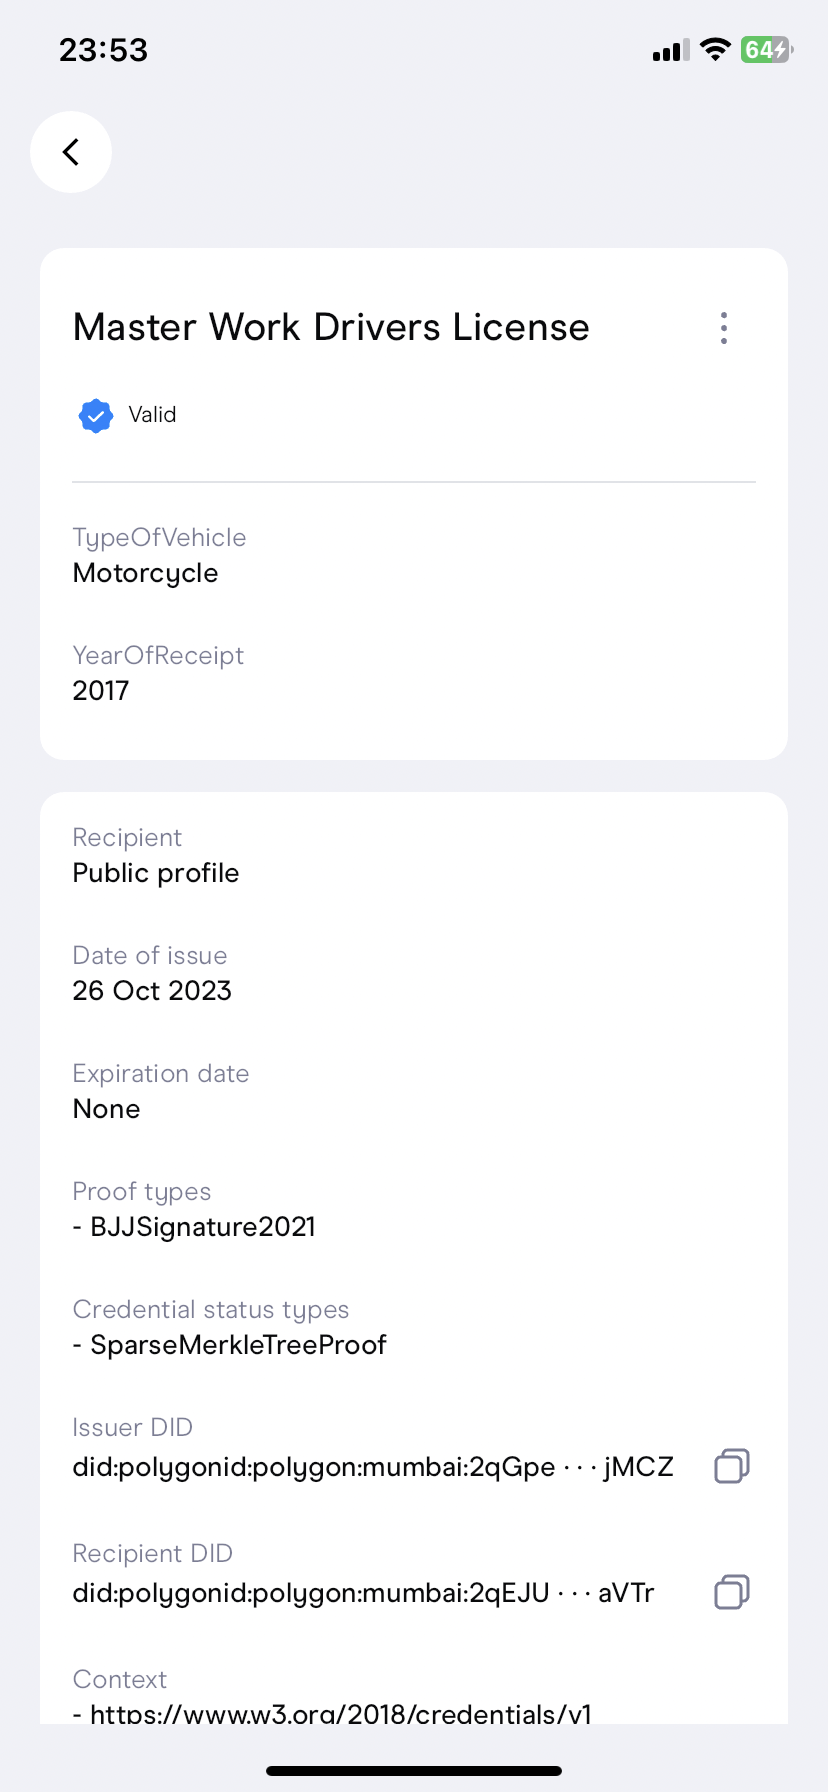
\includegraphics[scale=0.2]{media/appCredential}
	 	\caption{App Credential Beispiel}
	 	\label{fig:appCredential}
	 \end{figure}
	 
	 Es ist zu erkennen, dass die DID vom Issuer/Receiptient und die im CLI angegeben Attribute im Credential nachzuverfolgen sind.
	\end{itemize}
	 
\section{Der Verifier}
Der Verifier hat die Funktion die Credentials zu überprüfen. Hierbei wird zunächst überprüft, ob der Nutzer den Credential besitzt und ob er noch gültig ist, im Falle dass ein Auslaufdatum angegeben wurde oder der Credential widerrufen wurde. Drei Typen von Anfragen können gestellt werden:
\begin{itemize}
	\item Ohne Query: Entspricht einer Anfrage, die lediglich überprüft, ob der Credential existiert und valide ist
	\item Mit Query:
		\begin{itemize}
			\item Für Abfrage-Operatoren ungleich 'eq' (lt , gt, in, etc)
			\item Für Abfrage-Operation gleich 'eq'(entspricht ==). Dieser Typ von Anfragen wird auch als 'Selective Disclosure' bezeichnet.
		\end{itemize}
\end{itemize}
Gebaut werden können diese Anfragen mittels einem vom Polygon zur Verfügung gestellten Tool \cite{ID57}. Hierbei wird das Schema des Credentials geladen und über ein UI können die Attribute und Operatoren ausgewählt werden und ein JSON-Objekt wird als Ergebnis zurückgegeben.

Der oben beschriebe Query wird statisch im Programmcode festgehalten. \\
Über eine REST-API (gehostet auf port 8080) werden zwei Schnittstellen zur Verfügung gestellt:
\begin{itemize}
	\item /api: Dieser Endpunkt macht ist dafür zuständig den Request-Body zu bauen und zu speichern (wird später erneut benötigt). Zudem wird ein QRCode von dem Request abgespeichert, der mit der PolygonId-App gescannt werden kann. Der Request-Body sieht wie folgt aus:
	
\begin{lstlisting}[language=json,firstnumber=1]
{
	"from": "did:polygonid:polygon:mumbai:2qF57iujBWKeAGc2koCV56yW5S1SfPtFsCgDHzGRdW",
	"typ": "application/iden3comm-plain-json",
	"type": "https://iden3-communication.io/authorization/1.0/request",
	"body": {
		"reason": "Check if year of receipt is older than 2020",
		"callbackUrl": " https://df4c-165-1-191-123.ngrok-free.app/api/callback?sessionId=1",
		"scope": [
		{
			"id": 1,
			"circuitId": "credentialAtomicQuerySigV2",
			"query": {
				"allowedIssuers": ["*"],
				"type": "MasterWorkDriversLicense",
				"context": "https://ipfs.io/ipfs/QmTSd6saivXHysRopQdM1yswp2qyFwobL7fwuFpkVTS8gd",
				"credentialSubject": {
					"YearOfReceipt": {
						"$lt": 2020
					}
				}
			}
		}
		]
	}
}
\end{lstlisting}	
	\item /qr: dient als Endpunkt, um die QR-Codes zu lesen
\end{itemize}
Nachdem der Code von der App gescannt wurde, wird die Anfrage angezeigt. Ebenso wird die URL des Issuers angezeigt und der Name des Credentials. Der Holder initiert die Verifizierung durch das Drücken des "Approve"-Buttons. An dieser Stelle wird ein zk-Proof generiert und an den Verifier geschickt. Der Holder schickt hierfür einen POST-Request an die angegebene 'callbackURL'. An dieser Stelle führt der Server die tatsächliche Verifikation des zk-Proofs aus. Der Ablauf hierfür wird im folgenden Code beschrieben:
\begin{lstlisting}[language = JavaScript , frame = trBL , firstnumber = last , escapeinside={(*@}{@*)}]
	const ethURL = 'https://polygon-mumbai.g.alchemy.com/v2/PRIVATE_API_KEY';
	const contractAddress = "0x134B1BE34911E39A8397ec6289782989729807a4" //public verification contract adress
	
	const ethStateResolver = new resolver.EthStateResolver(
	ethURL,
	contractAddress,
	);
	
	const resolvers = {
		['polygon:mumbai']: ethStateResolver,
	};
	
	
	// fetch authRequest from sessionID
	const authRequest = requestMap.get(`${sessionId}`);
	
	// EXECUTE VERIFICATION
	let path_full = path.join(__dirname, './circuits-dir')
	const verifier = await auth.Verifier.newVerifier(
	{
		stateResolver: resolvers,
		circuitsDir: path_full,
		ipfsGatewayURL:"https://app.pinata.cloud/gateway/amethyst-official-duck-350?pinataGatewayToken=F5FDkLi66xtMWFQ0BCjZ1EGceaWSvbQ1uvkioaYqi9Iq4lSc8CRpMi-2EXVSa1f" // gateway used to save the ZK-Proof
	}
);
\end{lstlisting}
Man kann erkennen, dass Pinata nicht nur verwendet um die Schemata zu speichern, sondern auch als Gateway um die zk-Proofs abzulegen. Auch ist zu erkenne, dass eine URL für einen Polygon-Knoten notwendig ist, da zum einen auf Widerruf geprüft wird und zum anderen der unter 'contractAddress' gespeicherte Smart-Contract kontaktiert wird. Der Holder erhält im Anschluss die Information, dass mit Erfolg verifiziert wurde.

\subsection{On-Chain Verifikation}
An dieser Stelle sollte kurz erwähnt werden, dass es ebenso möglich wäre die Verifikation 'on-chain', also als Smart-Contract in der Blockchain ablaufen zu lassen. Analog dazu gibt es die Alternative auch den Issuer 'on-chain' zu implementieren.

//holder erklären
//interaktion
//integration von DLT in das Systemdesign

\section{Der Holder}
Der Holder ist die Komponente mit der geringsten Relevanz für diesen Prototypen. Es gibt jeweils eine App für Android und IOS, die folgende Funktionen haben \cite{ID58}:
\begin{itemize}
	\item SSI implementieren
	\item Credential entgegennehmen, speichern und warten
	\item zk-Proofs erstellen
	\item mit Issuer und Verifier kommunizieren
	\item Recovery-Funktion mittels 'seed-phrase'
\end{itemize}
Wenn ein Entwickler seinen eigenen 'Identity Wallet' implementieren möchte, hat er die Auswahl zwischen der Flutter-SDK (https://flutter.dev/) und einer Android SDK. Auch steht eine REST-API verschiedener Anbieter zur Verfügung, die Funktionen anbieten, die der Wallet benötigt, wie das Erstellen von Identitäten oder zk-Proofs.
Für diesen Prototypen wurde kein eigener Identity-Wallet implementiert, da der von Polygon-ID zur Verfügung gestellte Wallet bereits allen Anforderungen genügt und eine eigene Implementierung keinen Mehrwert liefert.

\section{Interaktion zwischen den Komponenten}
Um die Interaktion zwischen den Komponenten zu illustrieren wird folgende Grafik verwendet \ref{fig:trust}:

\begin{figure}[h]
	\centering
	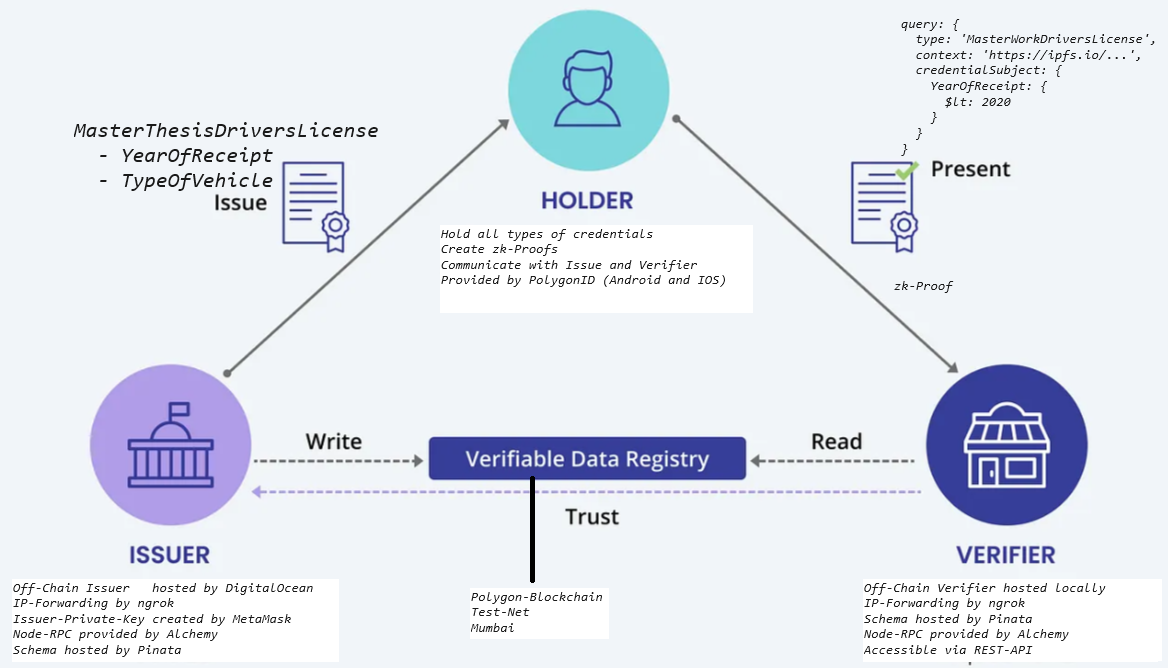
\includegraphics[scale=0.4]{media/trust}
	\caption{Interaktion zwischen den Komponenten}
	\label{fig:trust}
\end{figure}

Bei der Abbildung \ref{fig:trust} handelt es sich zunächst um das Konzept 'Triangle of Trust', dass mit den Details des Prototypen erweitert wurde. Unterhalb jeder der drei Komponenten werden technische Details zur Realisierung angegeben. Es ist zu erkennen, dass das Konzept abhängig davon ist, dass der Issuer korrekte Credentials angibt. In dem Szenario, dass der Issuer kompromittiert wurde oder bösartig ist würde folgende Situation eintreten:
\begin{itemize}
	\item Es werden fehlerhafte, unglaubwürdige erstellt.
	\item Das Schreiben von Credentials in die Blockchain gilt als Transaktion und daher würden Kosten entstehen
	\item Der Holder ist im Besitzt dieser falschen Credentials und könnte (evtl. sogar unwissentlich Identitätsdiebstahl begehen)
	\item Der Verifier vertraut der 'Verifiable Data Registry' und würde fehlerhafte Credentials als richtig attestieren
\end{itemize} 
Daher ist die Korrektheit des Issuer von elementarer Bedeutung. \\
Ein schematischer Ablauf von der Erstellung der Identität des Issuer hin zur erfolgreichen Verifikation eines Credential des Holder sieht wie folgt aus \ref{fig:kommunikation}.
\begin{figure}[h]
	\centering
	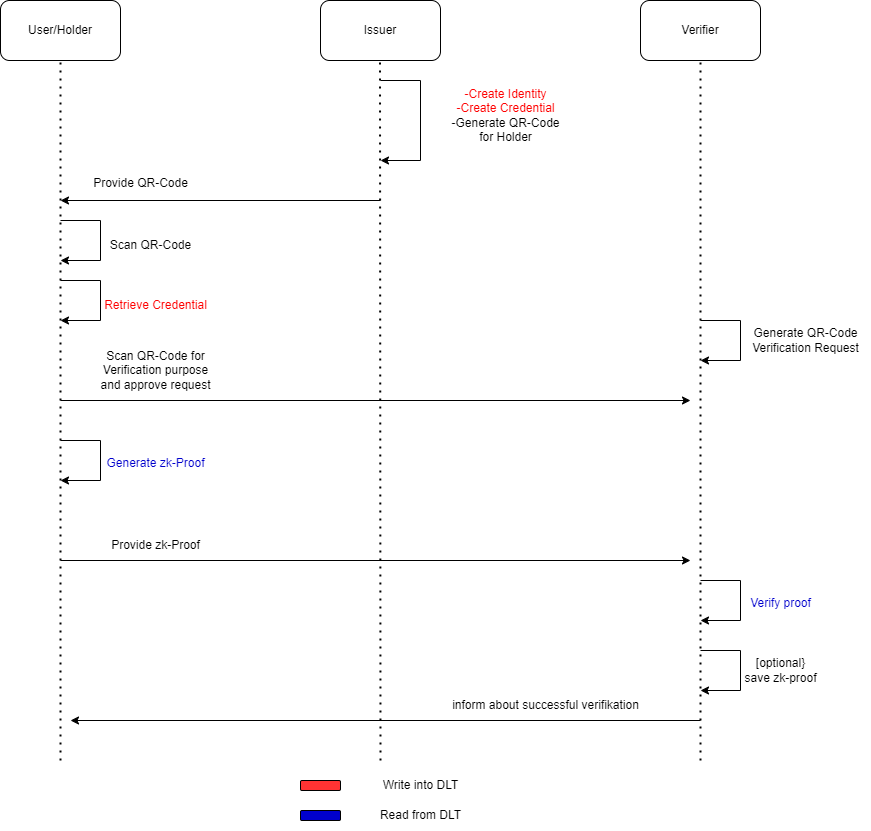
\includegraphics[scale=0.4]{media/kommunikation}
	\caption{Schematischer Ablauf des Prozesses}
	\label{fig:kommunikation}
\end{figure}
Rote Aktivitäten beinhalten Transaktionen in der Blockchain und blaue Aktivitäten beinhalten Schreibprozesse.
